\documentclass{beamer}
\beamertemplatenavigationsymbolsempty
\usecolortheme{beaver}
\setbeamertemplate{blocks}[rounded=true, shadow=true]
\setbeamertemplate{footline}[page number]
%
\usepackage[utf8]{inputenc}
\usepackage[english]{babel}
\usepackage{amssymb,amsfonts,amsmath,mathtext}

\usepackage{booktabs} % Allows the use of \toprule, \midrule and \bottomrule in tables
\usepackage{epigraph}
\usepackage{csquotes}
\usepackage{blindtext}

\usepackage{subfig}
\usepackage[all]{xy} % xy package for diagrams
\usepackage{array}
\usepackage{multicol}% many columns in slide
\usepackage{hyperref}% urls
\usepackage{hhline}%tables
% Your figures are here:
\graphicspath{{../figures/} }

%----------------------------------------------------------------------------------------------------------
\title[\hbox to 56mm{Influence of hyperparameters}]{Influence of hyperparameters on aggregating predictions of infinite number of experts}
\author[N.\,P.~Ivkin]{Sergey Kunin-Bogoiavlenskii}
\institute{Moscow Institute of Physics and Technology}
\date{\footnotesize
\par\smallskip\emph{Course:} My first scientific paper\par (Strijov's practice)/Group 125 %821, 813
\par\smallskip\emph{Expert:} R.\,D.~Zukhba
\par\smallskip\emph{Consultant:} A.\,V.~Zukhba
\par\bigskip\small 2024}

%----------------------------------------------------------------------------------------------------------
\begin{document}
%----------------------------------------------------------------------------------------------------------
\begin{frame}
\thispagestyle{empty}
\maketitle
\end{frame}

%-----------------------------------------------------------------------------------------------------
%\begin{frame}{Goal of research}
%..
%\end{frame}
%-----------------------------------------------------------------------------------------------------


%\begin{frame}
%\frametitle{What can be forecast?}
%%\begin{displayquote}
%%There are two kinds of forecasters: those who \\ don’t know, and those who don’t know they don’t know. \\ John Kenneth Galbraith
%%\end{displayquote}
%\epigraph{Tell us what the future holds, so we may know that you are gods.}{\textit{Isaiah 41:23}}
%%
%%\epigraph{There are two kinds of forecasters: those who \\ don’t know, and those who don’t know they don’t know.}{\textit{John Kenneth Galbraith}}
%%\blindtext
%\begin{itemize}
%\item Weather conditions
%\item Economic trends
%\item Technology advancements
%\item Consumer behavior
%\item Population growth
%\item Political elections outcomes
%
%\end{itemize}
%\end{frame}


%------------------------------------------------
\subsection{Goal of research} 

\begin{frame}
\frametitle{Goal of research}
\setlength\epigraphwidth{.45\textwidth}
\epigraph{Prediction is very difficult, especially if it's about the future.}{\textit{Niels Bohr}}
%\blindtext

\begin{block}{Goal}
Examining the influence of hyperparameters on the accuracy of the aggregation algorithm with an infinite number of experts
\end{block}


\begin{block}{Targets}
\begin{enumerate}
\item Time series generator implementation
\item Aggregating algorithm implementation
\item Experiments with various hyperparameters    
\end{enumerate}
\end{block}

%\begin{enumerate}
%\item Time series generator implementation
%\item Aggregating algorithm implementation
%\item Experiments with various hyperparameters    
%\end{enumerate}


\end{frame}
%-----------------------------------------------------------------------------------------------------

\begin{frame}{Literature}
    \begin{itemize}
    \item V.\,V’yugin, V.\,Trunov. 2023. Prediction of Locally Stationary Data Using Prediction with
Expert Advice. \url{http://www.jip.ru/2023/470-487-2023.pdf}
    
    \item N.\,Cesa-Bianchi, G.\,Lugosi. 2006. \\
    Prediction, Learning, and Games.
    \url{https://ii.uni.wroc.pl/~lukstafi/pmwiki/uploads/AGT/Prediction_Learning_and_Games.pdf}.
    
    \item Hyndman,\,R.\,J. \& Athanasopoulos,\,G., 2nd edition. 2018. Forecasting: Principles and Practice. \url{https://otexts.com/fpp2/}
%
%    \item Miles Cranmer, Sam Greydanus, Stephan Hoyer, Peter Battaglia, David Spergel, and Shirley Ho. Lagrangian neural networks. arXiv preprint arXiv:2003.04630, 2020.
%
%    \item Обработка датасета PAMAP2. https://github.com/andreasKyratzis/PAMAP2-Physical-Activity-Monitoring-Data-Analysis- and-ML/blob/master/pamap2.ipynb
  
    \end{itemize}
\end{frame}

%------------------------------------------------
\section{Problem statement} 
\subsection{Data} 

\begin{frame}
\frametitle{Problem statement}

\epigraph{There are two kinds of forecasters: those who \\ don’t know, and those who don’t know they don’t know.}{\textit{John Kenneth Galbraith}}

\textbf{Data}

It is assumed that there are multiple generators, whose structure is unknown to the predictors. These generators switch, producing a time series that is subdivided into a sequence of segments - areas of stationarity, which can be studied using machine learning methods. 

\bigskip
\textbf{Gerators implemented:}
\begin{itemize}
\item Linear 
\item ARMA
\end{itemize}




\end{frame}

%------------------------------------------------

\subsection{Terms} 

\begin{frame}
\frametitle{Problem statement}

\textbf{Terms}
\begin{itemize}
\item $X$ --- signals space
\item $Y$ --- responses space
\item $\mathcal{N}$ --- set of experts, indexed by natural numbers \\
\item $\mathsf{D}$ --- desicion space, to which predictions belong \\
\item $\lambda: \mathsf{D} \times \mathsf{Y} \rightarrow \mathbb{R}_+$ --- nonnegative loss function \\

\item $L^i_T = \sum\limits_{t = 1}^T l^i_t$ --- cumulative loss of expert $i$ during the first T steps \\
\item $H_T = \sum\limits_{t = 1}^T h_t$ --- master's cumulative loss during the first T steps \\
\item $R^i_T = H_T - L^i_T$ --- master's regret relative to the expert $i$ \\

\end{itemize}


\end{frame}

%------------------------------------------------

\setbeamertemplate{enumerate items}[default]
\subsection{Algorithm} 
\begin{frame}
\frametitle{Problem statement}

\textbf{Algorithm}

\bigskip
%
%\begin{enumerate}%[label={(\arabic*)}]
%\item Expert initialization
%\item Predictions
%\item Loss weights update
%\item Mixing weights update
%\end{enumerate}
FOR $t = 1, 2, \dots$:
\begin{enumerate}
\item Expert $f^t$ initialization
\item Experts' predictions $f_t^i = f_t^i(x_t),\ 1 \le i \le t$ 
\item Master's prediction evaluation $\gamma_t = \mathsf{Subst}(\mathbf{f_t}, \mathbf{\widehat{w}_t})$
\item Computation of master's loss $h_t = \lambda(p_t, y_t) $ and experts' losses $l_t^i$ 
%\item Modify experts' weights in two steps:

\item \textbf{Loss Update} weights modification
\item \textbf{Mixing Update} weights modification

\end{enumerate}

ENDFOR

\end{frame}


%------------------------------------------------
\section{Experiments} 
%\subsection{Hyperparameters} 

\begin{frame}
\frametitle{Experiments}
\begin{block}{Initialization weights}
Default weights: $w_1^i = \frac{1}{(i+1)\ln^2(i+1)}$

Experimental: $\frac{1}{i^\alpha}$, $\frac{1}{(i+1)\ln(i+1)\ln^2\ln(i+c)}, \frac{1}{e^i}$, etc.
%\begin{itemize}
%\item $\frac{1}{i^\alpha}$
%\item $\frac{1}{(i+1)\ln(i+1)\ln^2\ln(i+1)}$
%\end{itemize}
\end{block}

\begin{block}{Window size}
As the algorithm does not know the locations of generator switches, finding an optimal training window is also a challenge.
\end{block}

\begin{block}{Mixing update coefficients}
Default coefficient: $\alpha_t = \frac{1}{t+1}$

Experimental:  $\frac{1}{(t+1)^\beta}, \frac{1}{t+c}$, etc.

\end{block}

Metric - master's regret relative to the ideal expert (best partition)
\end{frame}

%------------------------------------------------

\begin{frame}


\frametitle{Table}
\begin{table}


\begin{tabular}{crr}
\toprule
train\_window & weight\_function & regret\\
\midrule
$5$ & $1 / ((i + 1) * ln^2(i + 1))$ & 224307.80 \\
$5$ & $1 / (i^{1.01})$ & 175677.06 \\
$10$ & $1 / ((i + 1) * ln^2(i + 1))$ &  142566.48 \\
$10$ & $1 / (i^{1.01})$ &  98022.98 \\
$20$ & $1 / ((i + 1) * ln^2(i + 1))$  & 135308.02 \\
$20$ & $1 / (i^{1.01})$ & 93522.27 \\
\bottomrule
\end{tabular}


\caption{Regret for different weight functions}
\end{table}



\end{frame}

%------------------------------------------------

\begin{frame}
\frametitle{Losses plot}
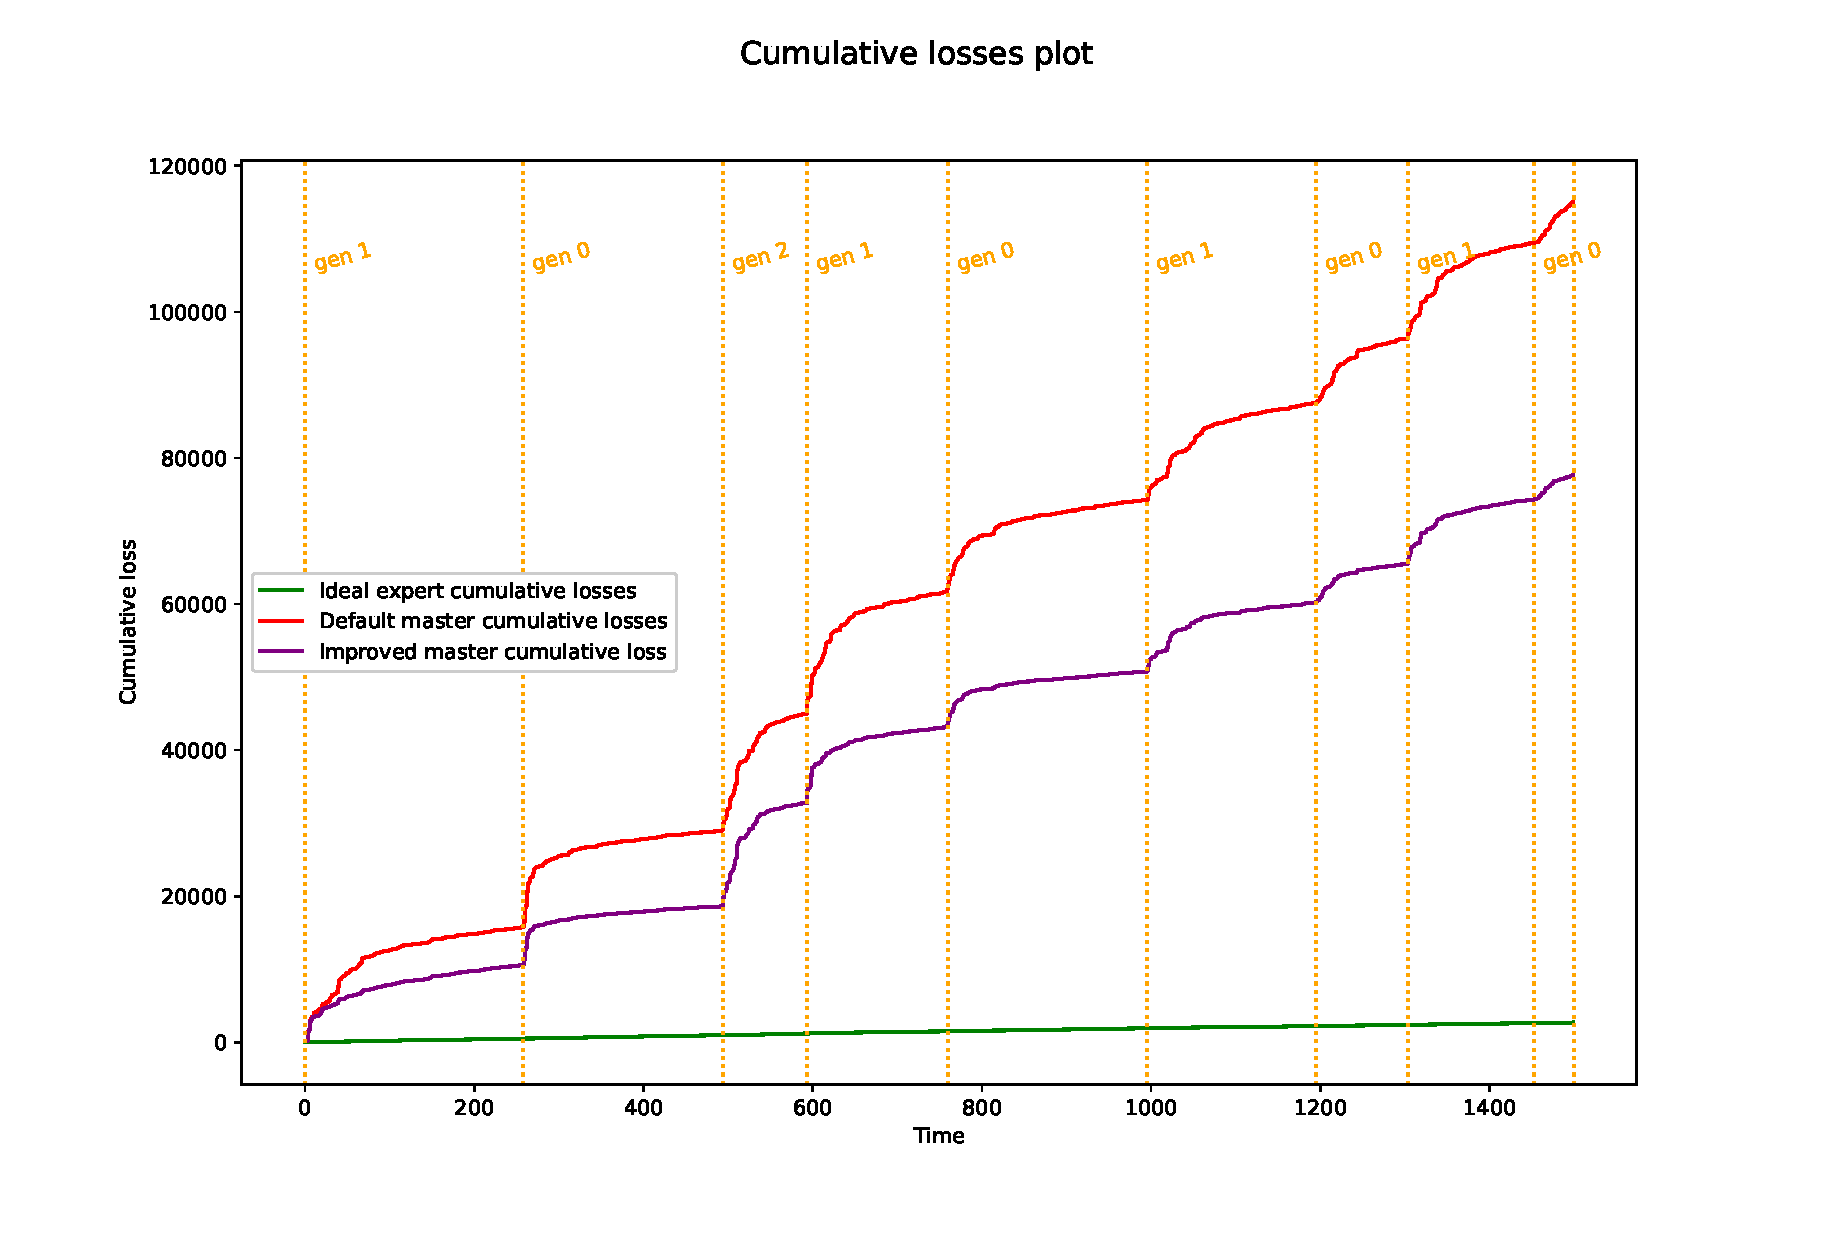
\includegraphics[width=1\linewidth]{improvement3}

%\begin{figure}
%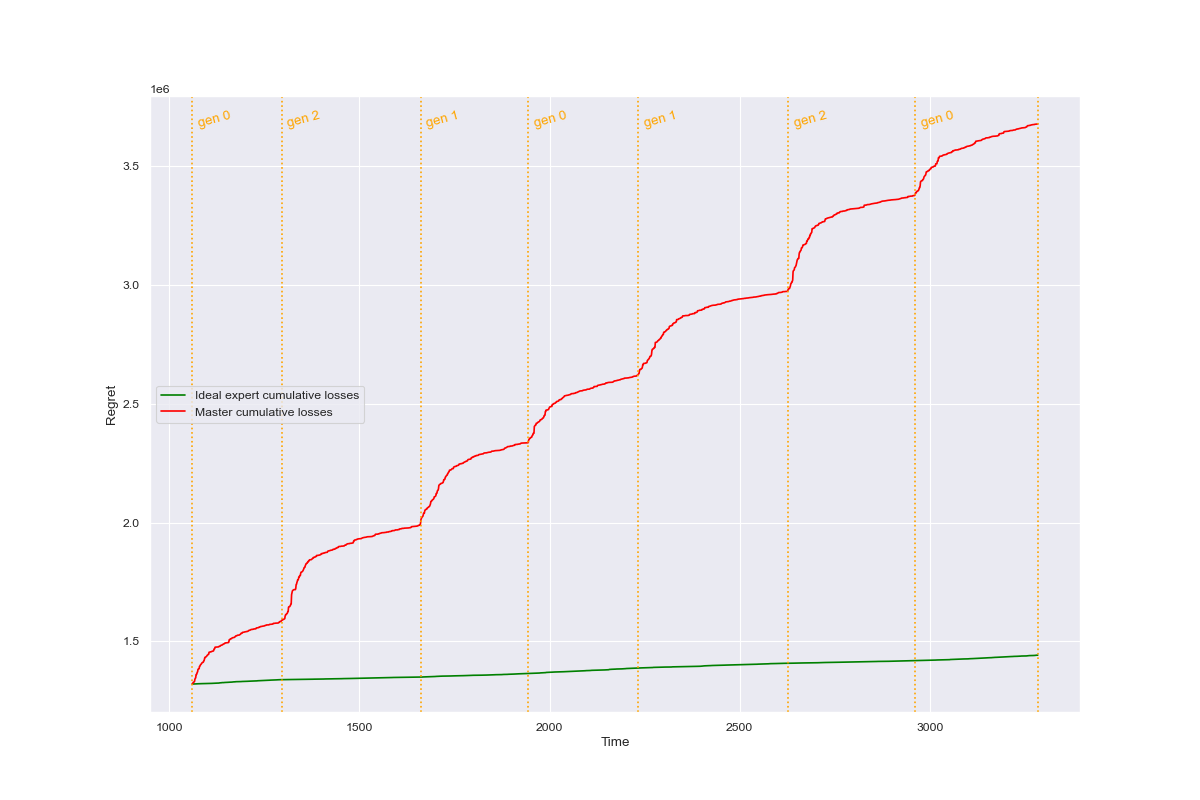
\includegraphics[width=1\linewidth]{fig}
%\end{figure}
\end{frame}

%------------------------------------------------

\begin{frame}
\frametitle{Conclusion}

\begin{block}
    
    Summary
        
    \begin{itemize}
  
        \item Generators and algorithm implemented
        \item Correctness of the algorithm veryfied
        \item A series of experiments conducted
        \item Enhanced weight function achieved
                
    \end{itemize}
    \end{block}    
    
    \begin{block}
    
    Further plans
    
    \begin{itemize}
    
        \item Run experiments on real data 
        \item Theoretically prove that the obtained function is the best.              
    \end{itemize}
    \end{block}

    
\end{frame}

%------------------------------------------------

\begin{frame}
\Huge{\centerline{The End}}
\end{frame}


%%----------------------------------------------------------------------------------------------------------
%\begin{frame}{Problem statement}
%..q
%\end{frame}
%%----------------------------------------------------------------------------------------------------------
%\begin{frame}{Solution}
%\begin{columns}[c]
%\column{0.6\textwidth}
%    Column 1
%\column{0.4\textwidth}
%    Column 2
%\end{columns}
%\end{frame}
%%----------------------------------------------------------------------------------------------------------
%\begin{frame}{Computational experiment}
%..
%\end{frame}
%%----------------------------------------------------------------------------------------------------------
%\begin{frame}{Conclusion}
%    \begin{block}{Forecast with hierarchical aggregation of}
%    \begin{itemize}
%        \item types of freight in
%        \item stations, regions, and roads,
%        \item for a day, week, month, and quarter.
%    \end{itemize}
%    \end{block}
%\end{frame}
%%----------------------------------------------------------------------------------------------------------
\end{document} 